\documentclass[a4paper,10pt,openright,openbib,twocolumn]{article}
%\usepackage[portuges]{babel}
\usepackage[T1]{fontenc}
\usepackage{ae}
\usepackage[utf8]{inputenc}
\usepackage[pdftex]{graphicx}
\usepackage{url}
\usepackage{listings}
\usepackage{verbatim}
\usepackage{enumerate}
\usepackage[pdftex, bookmarks, colorlinks, linkcolor=black, urlcolor=blue]{hyperref} 
\usepackage[a4paper,left=2.5cm,right=2.5cm,top=3.5cm,bottom=3.5cm]{geometry}
\usepackage{colortbl}
\usepackage[margin=10pt,font=small,labelfont=bf]{caption}
\usepackage{mdwlist}
\usepackage{cleveref}
\usepackage{epsfig}

\usepackage{multicol}
\usepackage{appendix}


\setlength{\parindent}{0cm}
\setlength{\parskip}{2pt}


\begin{document}

\begin{multicols}{2}
\title{Roofline and Matrix Multiplication PAPI Analysis}
\author{
    Brito, Rui\\
    PG22781\\
    Department of Informatics\\
    University of Minho\\
    ruibrito666@gmail.com
  \and
    Alves, José\\
    PG22765\\
    Department of Informatics\\
    University of Minho\\
    zealves.080@gmail.com
}
\date{}
\maketitle
\end{multicols}

\begin{abstract}
	This paper describes the roofline\cite{roofline} analysis of two different machines. The roofline consists in a theoretical performance model that provides visual insights on floating point computing performance. This model relates processor performance to off-chip memory traffic, giving a upper bound on performance of a kernel depending on its operational intensity. There is also a study of a matrix dot product using PAPI(Performance Application Programming Interface)\cite{papi}. With PAPI we are able to use the low-level hardware counters to identify the most accessed areas of our memory hierarchy as well as the operations made by running software.  
\end{abstract}

\section{Introduction}
The importance of a system’s characterization is due to the need of understanding the limitations of a system, in order to make the necessary optimizations to obtain the maximum performance of a system. In order to provide a easy-to-understand performance model for floating-point programs, the Roofline Model was created. The Roofline indentifies a theoretical upper bound on performance on a kernel that relates if a certain opetional intensity is memory-bound, dependant on accesses of memory, or computational-bound, dependant on floating-point operational units. To comprehend the influence of different components and certain architecture characteristics a number of ceilings, both computational and memory driven, may be added. Since the Roofline Model is better understood with a case study, a matrix multiplication problem was proposed to present the theoretical limitations of the algorithm through the model. To specify the problem in the Roofline model, a series of values were obtained from the hardware counters through PAPI(Performance Application Programming Interface). PAPI allow us to reach the low-level hardware counters and obtain information from components accessed by the software running. 

%% Roofline%%
\section{Roofline}
\subsection{Machine Profiles}
The machines used for this study were an Apple MacBook Pro late 2008 and a 2010 HP dv6-2190ep.
Information about the machines was gathered from various *NIX tools (e.g \emph{/proc/cpuinfo}, \emph{/proc/meminfo}, \emph{dmidecode} and \emph{sysctl}) and from the web (e.g. \emph{Intel Ark} and \emph{Crucial}). To calculate cache and main memory bandwidth we used the tool \emph{bandwidth} \footnote{http://zsmith.co/bandwidth.html}.

\subsubsection{Performance Peaks}
In order to calculate the rooflines, we needed the Floating-Point(FP) Performance Peak and the Memory Bandwidth's Peak. 
To attain the FP Performance Peak we solve the following formula:

$$\mathrm{GFlop/s_{max}} =  \#_{\mathrm{cores}} \times f_{\mathrm{clock}} \times \#_{\mathrm{SIMD}}$$

MacBook Pro FP Performance Peak:
$$\mathrm{GFlop/s_{max}} =  2 \times 2.8 \times 8
						 =  44.8 GFLOPS\\s$$
HP Pavillion FP Performance Peak:
$$\mathrm{GFlop/s_{max}} =  4 \times 1.6 \times 8
						 =  51.2 GFLOPS\\s$$
\\
\\
To calculate de Memory Bandwidth Peak we solve the following formula:

$$\mathrm{BW_{max}} =  \#_{\mathrm{channels}} \times mem_{\mathrm{clock}} \times bus_{\mathrm{bandwidth}}$$
 
MacBook Pro Memory Bandwidth Peak:
$$\mathrm{GFlop/s_{max}} =  2 \times 1067 \times 64
						 =  17.072 GB\\byte$$
HP Pavillion Memory Bandwidth Peak:
$$\mathrm{GFlop/s_{max}} =  2 \times 1333 \times 64
						 =  21.328 GB\\byte$$

\subsubsection{Specifications}
The specifications for the MacBook Pro are displayed on \autoref{tab:mbp}. \\
\small{It should be noted that L1 Access Bandwidth refers to 128-bit sequential reads}\\

\section{sdjfdsfhsdk} % (fold)
\label{sec:sdjfdsfhsdk}

% section sdjfdsfhsdk (end)
	

\tabcolsep=0.11cm
\begin{table}[!htp]
	\footnotesize
		\begin{tabular}{lrl}
			\hline 
			\textbf{Manufacter:} & Apple \\
			\hline \\
			\textbf{Model:} & MacBook Pro late 2008 \\
			\hline 
			\textbf{Processor} & & \\
			Manufacturer: & Intel & \\
			Arch: & Core & \\
			Model: & Core 2 Duo T9600 & \\
			Cores: & 2 & \\
			Clock Frequency: & 2.80 GHz & \\
			FP Performance's Peak: & 44.8 GFlops/s & \\
			\hline 
			\textbf{Cache} & & \\
			Level: & 1 & \\
			Size: & 32KB + 32KB & \\
			Line Size: & 64 B & \\
			Associative: & 8-way & \\			
			L1 Access Bandwidth: & 40 GB/s & \\
			\\
			Level: & 2 & \\
			Size: & 6 MB & \\
			Line Size: & 64 B & \\
			Associative: & 24-way & \\
			\hline 
			\textbf{RAM} \\
			Type: & SDRAM DDR3 PC3-8500 & \\
			Frequency: & 1067 MHz & \\
			Size: & 4 GB & \\
			Num. Channels: & 2 & \\
			Latency: & 13.13 ns & \\
		\end{tabular}
		\caption{MacBook Pro late 2008 specifications}
		\label{tab:mbp}
\end{table}
The specifications for the HP dv6-2190ep are displayed on \autoref{tab:hp}. \\
\begin{table}[!htp]
	\footnotesize
		\begin{tabular}{lrl}
			\hline 
			\textbf{Manufacter:} & HP \\
			\hline 
			\textbf{Model:} & Pavillion dv6-2190ep \\
			\hline 
			\textbf{Processor} & & \\
			Manufacturer: & Intel & \\
			Arch: & Nehalem & \\
			Model: & i7-720QM & \\
			Cores: & 4 & \\
			Clock Frequency: & 1.60 GHz & \\
			FP Performance's Peak: & 51.2 GFlops/s & \\
			\hline 
			\textbf{Cache} & & \\
			Level: & 1 & \\
			Size: & 32KB + 32KB & \\
			Line Size: & 64 B & \\
			Associative: & 4/8-way & \\
			L1 Access Bandwidth: & 22 GB/s & \\
			\\
			Level: & 2 & \\
			Size: & 256 KB & \\
			Line Size: & 64 B & \\
			Associative: & 8-way & \\
			\\
			Level: & 3 & \\
			Size: & 6 MB & \\
			Line Size: & 64 B & \\
			Associative: & 12-way & \\
			\hline 
			\textbf{RAM} \\
			Type: & SDRAM DDR3 PC3-10600 & \\
			Frequency: & 1333 MHz & \\
			Size: & 4GB & \\
			Num. Channels: & 2 & \\
			Latency: & 13.5 ns & \\
		\end{tabular}
		\caption{HP Pavillion dv6-2190ep specifications}
		\label{tab:hp}
\end{table}


\subsection{Roofline Model}
\subsubsection{MacBook Pro Roofline}
\begin{figure}[!htp]
	\centering
	\begin{minipage}[t]{\columnwidth}
		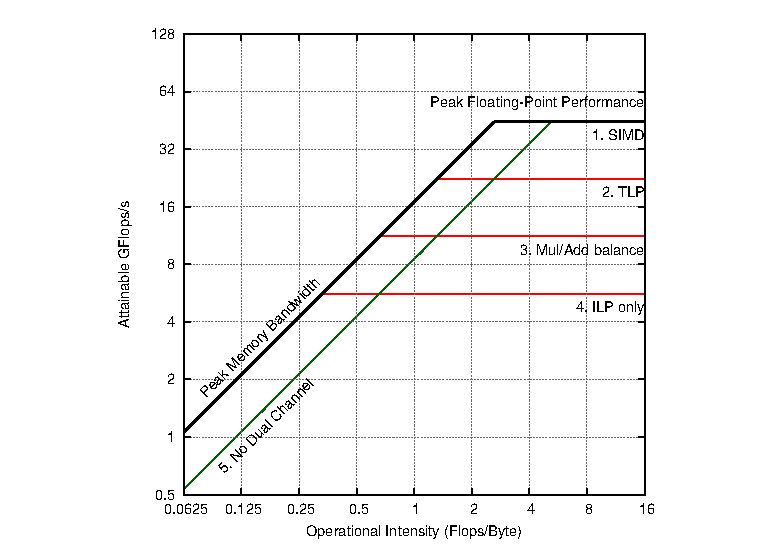
\includegraphics[width=\textwidth]{images/roofline_mbp.eps}
		\caption{Mackbook Pro late 2008 \label{fig:roofline1}}
	\end{minipage}
\end{figure}
\subsubsection{HP Pavillion Roofline}
\begin{figure}[!htp]
	\centering
	\begin{minipage}[t]{\columnwidth}
		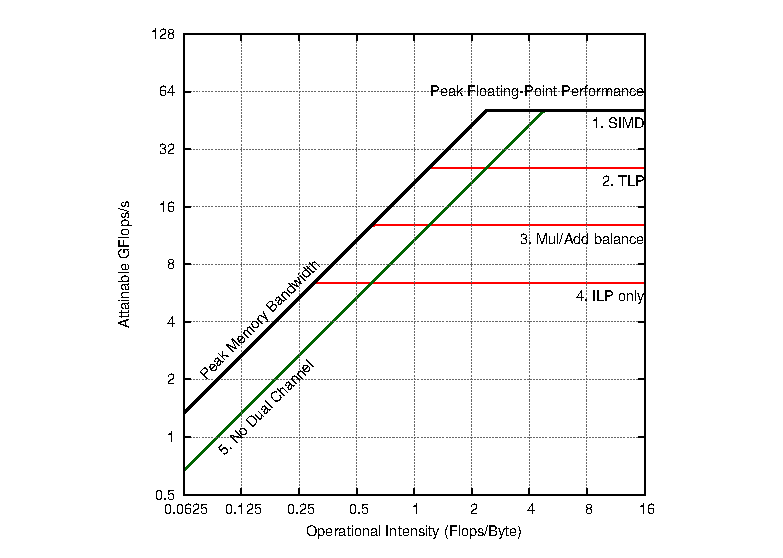
\includegraphics[width=\textwidth]{images/roofline_hp.eps}
		\caption{HP Pavillion dv6-2190ep Roofline \label{fig:roofline2}}
	\end{minipage}
\end{figure}

\section{PAPI Case Study}
\subsection{Problem}
The case study of this report, is to analyse the performance of a \textbf{matrix dot product} algorithm, \begin{equation}Matrix A * Matrix B = Matrix C\end{equation} wich contains a triple nested loop with the indexes i,j and k(line,column and position). A naive implementation of this algorithm will provide, at best, very weak performance, since for every iteration of the j loop the whole current line of the matrix will be brought to cache (if it fits), however, since the j loop sweeps columns, this proves to be very inefficient. Our aim was to minimize this inefficiency.

\subsection{Algorithm Analysis}
The implementation produced to calculate the matrix multiplication was coded in C and compiled with Optimization level 3 (-O3, so the compiler can explore SIMD extensions).
The naive algorithm of matrix multiplication is presented here, in order to better understand the problem at hand.
\small
\begin{verbatim}
for (i = 0; i < size; i++) {
    for (j = 0; j < size; j++) {
        for(k = 0; k < size; k++) {
                acc += matrixA[i][k] * 
                         matrixB[k][j];				
            }		
            matrixC[i][j] = acc;	
            acc = 0;
        }
    }
\end{verbatim}

And, for completeness' sake, here's the optimized version. Note that the matrix \emph{tMatrix} is transposed so we can take advantage of a unit stride. 
\small
\begin{verbatim}
    for (i = 0; i < size; i++) {
        for (j = 0; j < size; j++) {
            for(k = 0; k < size; k++) {
                acc += matrixA[i][k] * 
                           tMatrix[j][k];				
            }		
            matrixC[i][j] = acc;	
            acc = 0;
        }
    }		
\end{verbatim}

Two versions of the program were run, one with the original matrixB and other where matrixB is transposed. With this second version, it is expected for the algorithm to access a continous memory space, thus leveraging unit stride, increasing overall performance while reducing memory accesses (due to the reduced miss rate).

\subsection{Tests}
\subsubsection{Methodology}
To measure the algorithm's perfomance, hardware counters were used. To gather information from these counters we used \emph{PAPI}(Performance API). This tool alowed us to measure (among others) the following counters:
\begin{description}
\item[PAPI \_TOT\_CYC] Total number of cycles;
\item[PAPI \_TOT\_INS] Instructions completed;
\item[PAPI \_LD\_INS] number of load instructions;
\item[PAPI \_SR\_INS] number of store instructions;
\item[PAPI \_FP\_OPS] Floating point operations;
\item[PAPI \_FP\_INS] Floating point instructions;
\item[PAPI \_L1\_DCA] L1 data cache accesses;
\item[PAPI \_L1\_DCM] L1 data cache misses;
\item[PAPI \_L2\_DCA] L2 data cache accesses;
\item[PAPI \_L2\_DCM] L2 data cache misses;
\item[PAPI \_L3\_DCA] L3 data cache accesses;
\end{description}

Moreover, all tests were run on a dedicated execution of the algorithm with process niceness set to -20 (\emph{nice -n -20}) to ensure that essential machine time wasn't being spent on some other task. Also, to minimize overhead, OS Widgets and network were disabled. To decrease the chance of human error, the execution of all tests was "commanded" by a bash script. This script was also responsible for checking the 5\% error margin, and, in case it wasn't satisfied, re-running the tests.


\subsubsection{Test Cases}

All four tests, presented below, were chosen to run in the two different version(normal and transpose). Each test was run four times, with the best execution time being selected within a margin of 5\%.
\begin{table}[!htp]
	\center{
	\begin{tabular}{lrlrlrl}
		\hline
		\textbf{Memory} & \textbf{Size} & \textbf{Matrix Size} \\
		\hline
		L1 & 30 KB & 50 \\
		L2 & 255 KB & 146 \\
		L3 & 3 MB & 500 \\
		RAM & 7.68 MB & 800 \\
		\hline
	\end{tabular}
	\caption{Test cases}
	\label{tab:testcases}
	}
\end{table}
\subsection{Results}
\subsubsection{Cache Analysis}

 To measure the data cache misses the counters PAPI\_L1\_DCM and PAPI\_L2\_DCM were used. Each test fits in a different memory hierarchy level(L1, L2, L3 and RAM). (Note that test suffixed with a 0 mean unoptimized version, while those suffixed with a 1 mean, optimized version).

\begin{figure}[!htp]
	\centering
	\begin{minipage}[t]{\columnwidth}
		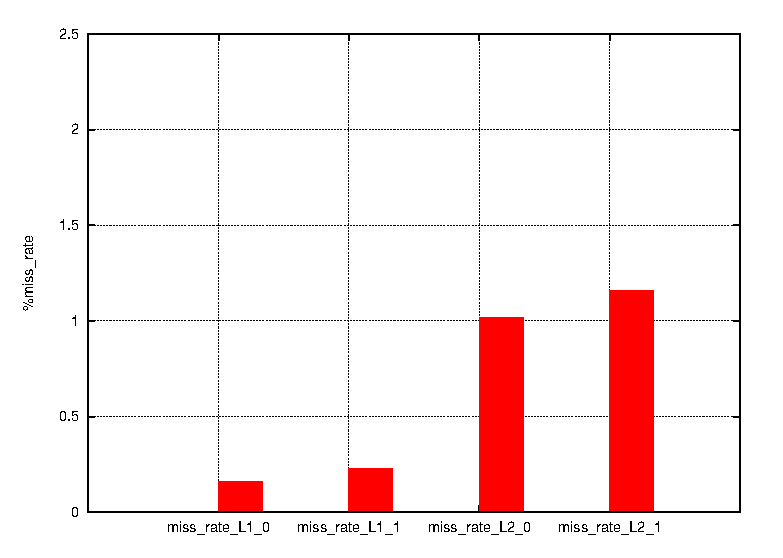
\includegraphics[width=\textwidth]{images/caches.eps}
		\caption{Percentage of Cache Misses \label{fig:cachel1}}
	\end{minipage}
\end{figure}

The above graphic shows an increase of percentage of misses with the optimized version, they are misleading. The next graph shows that although the percentage of misses increased, the total of misses didn't because the number of accesses also droped.

\begin{figure}[!htp]
	\centering
	\begin{minipage}[t]{\columnwidth}
		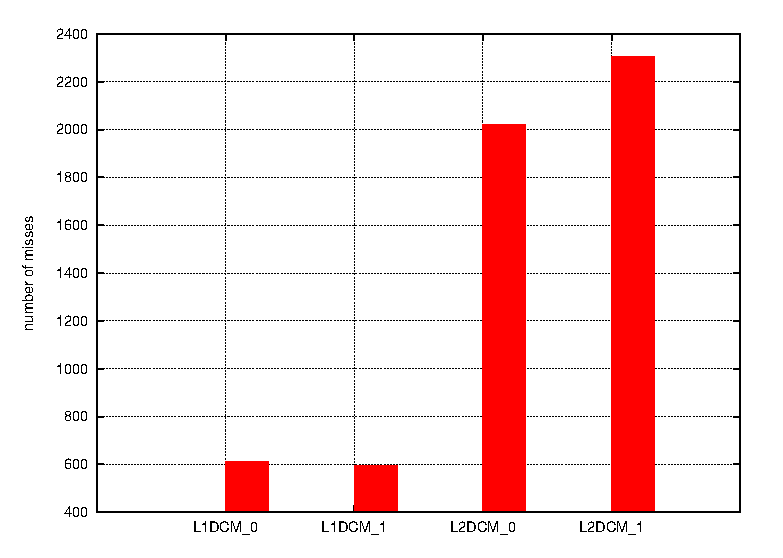
\includegraphics[width=\textwidth]{images/misses.eps}
		\caption{Number of Cache Misses \label{fig:cachel1}}
	\end{minipage}
\end{figure} 

Usage of both levels of cache was estimated with specific counters. PAPI\_L1\_DCA and PAPI\_L2\_DCA provided the number of data accesses to the caches.

Before the results were out, it was expected a decrease of cache accesses from version one to version two of the algorithm.

\begin{figure}[!htp]
	\centering
	\begin{minipage}[t]{\columnwidth}
		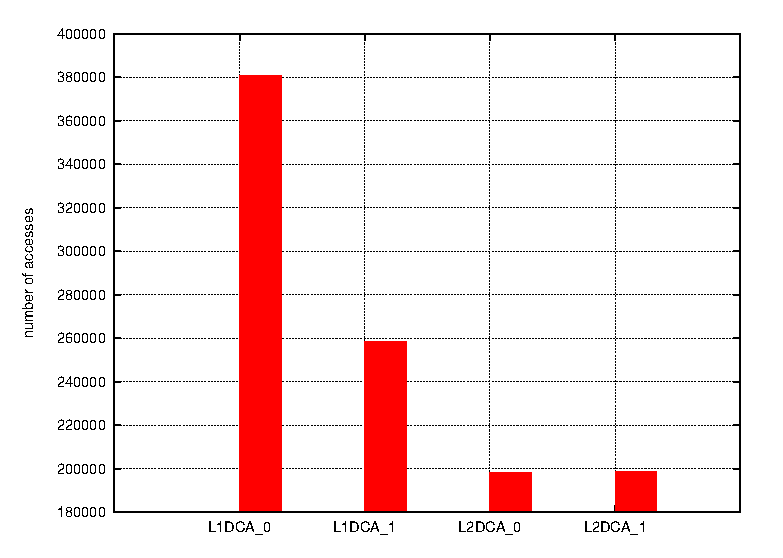
\includegraphics[width=\textwidth]{images/totals.eps}
		\caption{Number of Memory Accesses \label{fig:cachel1}}
	\end{minipage}
\end{figure}

As we can see, the number of access to cache drops significantly from the first version to the second version while running with the L1 Cache Test. Though in the second test, the L2 Cache, the number of accesses slightly increased.\\

For more palpable values, the following table shows the execution times.

\begin{table}[!htp]
	\center{
	\begin{tabular}{lrlrlrl}
		\hline
		\textbf{Test} & \textbf{Time ($\mu$s)} \\
		\hline
		L1\_0  &  271.091 \\
		L1\_1  &  254.000 \\
		L2\_0  &  6983.450 \\
		L2\_1  &  6629.000 \\
		L3\_0  &  521429.0 \\
		L3\_1  &	260535.0 \\
		RAM\_0 &  6.60003e+06 \\
		RAM\_1 &	3 1.08117e+06 \\
		\hline
	\end{tabular}
	\caption{Execution Times}
	\label{tab:execTimes}
	}
\end{table}

As it can be seen, the best improvements are seen in cache level 3 and in the main memory.

\subsection{Going Even Further}
The transposed matrix optimization, while showing improvements, it still is far away from the desired peak performance. Apart from enabling and/or taking advantage of all the features shown in the roofline model, implementing the algorithm in a way so that it uses blocks, would dramatically improve performace\cite{caqa}. But that isn't this paper's goal, we just wanted to let the readers know that there is still much to improve on. 

\begin{thebibliography}{99}
\bibitem{roofline}
	\texttt{\small
	Roofline: An insightful Visual Performance Model for Floating-Point Programs and Multicore Architectures}	\\
	\emph{Samuel Webb Williams, Andre Waterman, David A. Patterson}	\\
	23th November 2012

\bibitem{papi}
	\texttt{\small
	Experiences and Lessons Learned with a Portable Interface to Hardware Performance Counters}	\\
	\emph{Jack Dongarra, Kevin London, Shirley Moore, Philip Mucci, Daniel Terpstra, Haihang You, Min Zhou}	\\	


\bibitem{caqa}
	\texttt{\small
	Computer Architecture: A Quantitative Aproach, 5th Ed.}	\\
	\emph{John L. Hennesy, David A. Patterson}	\\	

\bibitem{ark}
	\texttt{\small
	http://ark.intel.com/}

\bibitem{crucial}
	\texttt{\small
	http://www.crucial.com}

\bibitem{wiki}
	\texttt{\small
	httt://www.wikipedia.com}




\end{thebibliography}

\appendix
\appendixpage
\section{CUDA Implementation}
Furthermore, an implementation of this algorithm was done using the GPU. We used the MacBook Pro referred earlier which has an NVIDIA GeForce 9600M GT with a compute capability of 1.1. The GPU kernel is has follows:

\begin{verbatim}
	__global__ void dotProduct( float* matrixA, float* matrixB, 
	                              float* matrixC, int n) {
 
   int j = blockIdx.x * blockDim.x + threadIdx.x;
   int i = blockIdx.y * blockDim.y + threadIdx.y;
      
   float value = 0;
   int k;
   for (k = 0; k < n; k++) {  	    	 
      value += matrixA[i * n + k] * matrixB[k * n + j];           
   }  

   matrixC[i * n + j] = value;
}
\end{verbatim}

To measure it's performance we used the NVIDIA command line profiler which read hardware counters from the GPU. Table \ref{tab:cuda} shows those results for a matrix of size (20x20). Using NVIDIA's own \emph{matrixMulCUBLAS}, we got the peak performance for this particular GPU which is 14.48 Gflops. With our naive algorithm we achieved 3.44 Gflops. There should probably be another Roofline taking the GPU into account, with ceilings such as SW Prefetching, Shared Memory, Memory Coalescing, NUMA allocation and usage, etc...

\begin{table}[!htp]
	\footnotesize
	\center{
	\begin{tabular}{lrlrlrl}
		\hline
		\textbf{method} & \textbf{gputime} & \textbf{cputime} & \textbf{instructions} \\
		\hline		
			memcpyHtoD & 6.912 & 26.669 & - \\
			memcpyHtoD & 6.048 & 17.427 & - \\
			dotProduct & 64.960 & 94.172 & 2237 \\
			memcpyDtoH & 5.920 & 42.166 & - \\
		\hline
	\end{tabular}
	\caption{Cuda Profile}
	\label{tab:cuda}
	}
\end{table}

\section{Images}
\begin{figure*}[!htp]
	\centering
	\begin{minipage}[t]{\linewidth}
		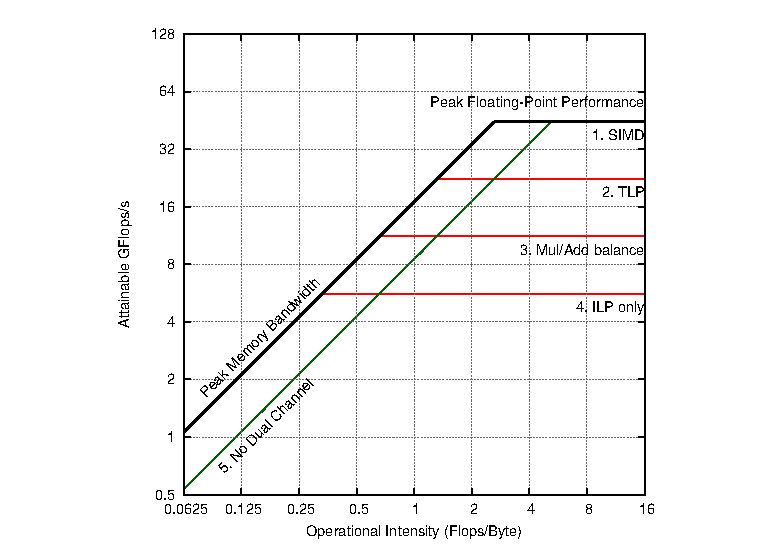
\includegraphics[width=\linewidth]{images/roofline_mbp.eps}
		\caption{Mackbook Pro late 2008 }
	\end{minipage}
\end{figure*}
\begin{figure*}[!htp]
	\centering
	\begin{minipage}[t]{\linewidth}
		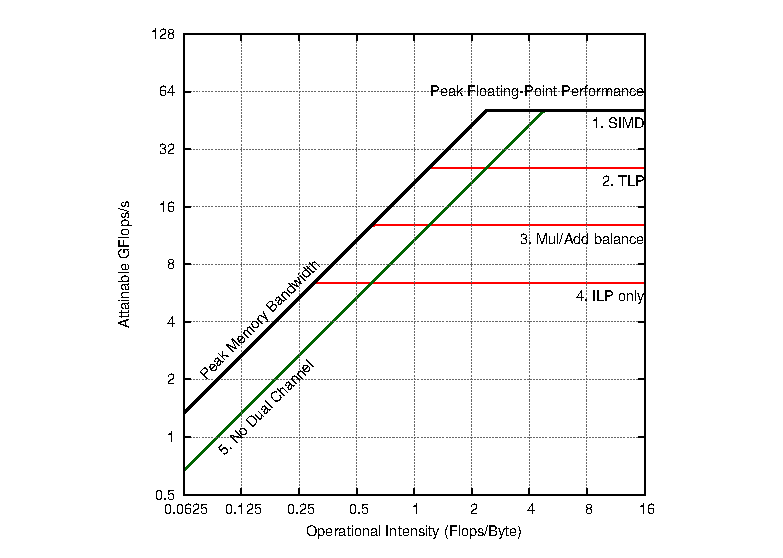
\includegraphics[width=\linewidth]{images/roofline_hp.eps}
		\caption{HP Pavillion dv6-2190ep Roofline }
	\end{minipage}
\end{figure*}

\begin{figure*}[!htp]
	\centering
	\begin{minipage}[t]{\linewidth}
		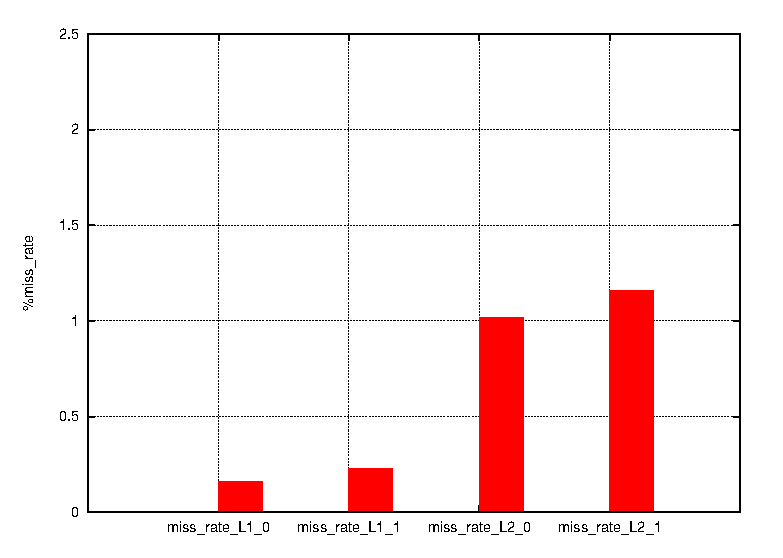
\includegraphics[width=\linewidth]{images/caches.eps}
		\caption{Percentage of Cache Misses }
	\end{minipage}
\end{figure*}
\begin{figure*}[!htp]
	\centering
	\begin{minipage}[t]{\linewidth}
		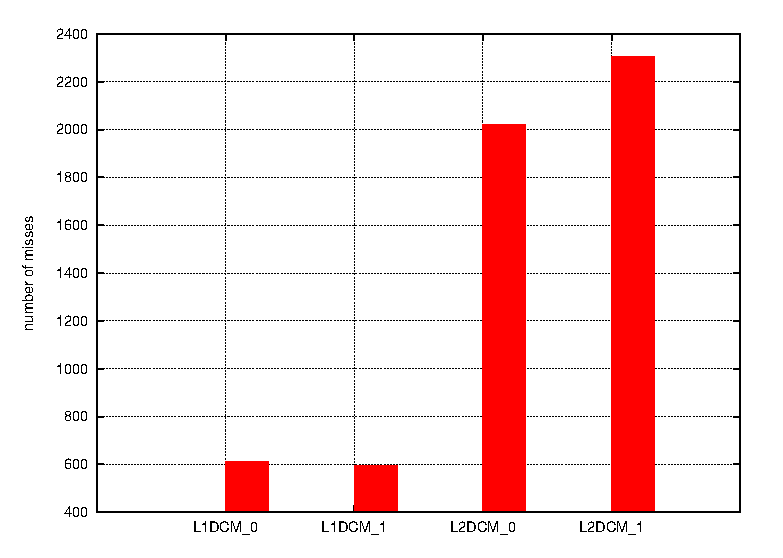
\includegraphics[width=\linewidth]{images/misses.eps}
		\caption{Number of Cache Misses }
	\end{minipage}
\end{figure*} 
\begin{figure*}[!htp]
	\centering
	\begin{minipage}[t]{\linewidth}
		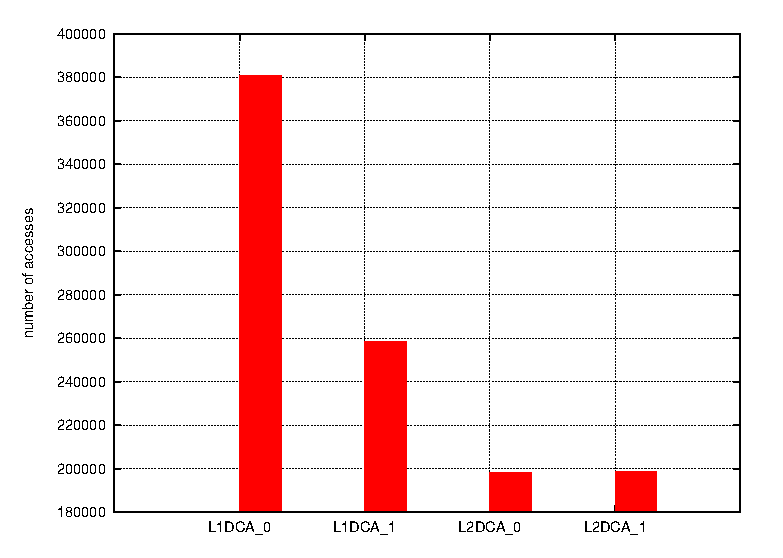
\includegraphics[width=\linewidth]{images/totals.eps}
		\caption{Number of Memory Accesses }
	\end{minipage}
\end{figure*}



\end{document}
